
This suite of tools satisfies the necessities (i)~to search the OEIS offline
and to automate searches, (ii)~to work in the console and with notebooks and
(iii)~to have an unified working environment where a single, general purpose,
programming language is used to integrate the OEIS with a symbolic algebra
system. Here, \textit{Python} plays the role of the glue language, relying
on the module \textit{Sympy} for symbolic computations.

\section{The Crawler}

The script \verb|crawling.py| fetches sequences recursively where the union of
cross refs sections defines the fringe to fetch.  It features no threads, no
race conditions, no data sync; on the contrary, it lies on \textit{async/await}
Python primitives only for pure asynchronous computation and the implementation
boils down to $300$ lines of Python code.  In the end, it allows us to cache
portions of the OEIS to speed up repeated lookups and to restart from the cache
already fetched. 

The script presents a help message to explain itself:
\VerbatimInput[fontsize=\small]{OEIS/crawler-help.txt}

We illustrate a typical session where we start from scratch; first of all, we
download two important and nice sequences, namely those corresponding to the
Fibonacci and Catalan numbers, respectively:
\VerbatimInput[fontsize=\small]{OEIS/crawler-fetching-command.txt}
we check the content of our cache with
\VerbatimInput[fontsize=\small]{OEIS/crawler-status.txt}
and display raw data displaying pure \textit{json} content about
the sequence $A000045$, using a simple printer provided by the Python module
\verb|json.tool|:
\VerbatimInput[fontsize=\small]{OEIS/crawler-A000045-chunk.txt}
Moreover, we can restart our downloading process from where we left before
\VerbatimInput[fontsize=\small]{OEIS/crawler-restarting.txt}
checking that new sequences are actually saved
\begin{Verbatim}[fontsize=\small]
$ python3.6 crawling.py 
50 sequences in cache ./fetched/
354 sequences in fringe for restarting
\end{Verbatim}

Looking at the implementation, the \verb|reader| class has the responsibility
to wait asynchronously for incoming data the \verb|read| coroutine:
\inputminted[fontsize=\small,stripnl=false,firstline=28,lastline=39]
    {python}{deps/oeis-tools/src/crawling.py}

The \verb|fetcher| class has the responsibilities (i)~to create a socket with
OEIS server, (ii)~to establish a working connection, (iii)~send an http
\verb|GET| request for the desired sequence, (iv)~wait for the fetching process
completes and (v)~to close the socket and signal that the work ends
successfully.
\inputminted[fontsize=\small,stripnl=false,firstline=41,lastline=86]
    {python}{deps/oeis-tools/src/crawling.py}

The \verb|crawler| class has the responsibilities 
(i)~to keeps a queue of task, one for each candidate sequence, 
(ii)~to put each ready task into a scheduling process to get executed and
(iii)~to reclaim memory from completed task and to deque them.
\inputminted[fontsize=\small,stripnl=false,firstline=89,lastline=117]
    {python}{deps/oeis-tools/src/crawling.py}

Finally, the function \verb|oeis| puts all together and it is the main
interface exported by the \verb|crawling| module:
\inputminted[fontsize=\small,stripnl=false,firstline=195,lastline=221]
    {python}{deps/oeis-tools/src/crawling.py}

\section{The (Pretty) Printer}

The script \verb|pprinting.py| provides a proxy for searching in the OEIS, it
shows exactly the same content you get from usual search interface on
http://oeis.org; additionally, it provides (i)~tabular representation of
\verb|data| sections in \textit{one and two dimensions} using list and matrix
notation, respectively, (ii)~filtering capabilities on most result's sections
and (iii)~takes advantage of cached sequences built by the crawler.

The script presents a help message to explain itself:
\VerbatimInput[fontsize=\small]{OEIS/pprinting-help.txt}

\VerbatimInput[fontsize=\small]{OEIS/pprinting-A000045.txt}

The following command pretty prints (i)~the first 3 results from cached
sequences, (ii)~ranking them according to the most recent access time,
(iii)~reporting data only and (iv)~limiting up to 10 elements for linear
sequences:
\VerbatimInput[fontsize=\small]{OEIS/pprinting-data-only.txt}

\VerbatimInput[fontsize=\small]{OEIS/pprinting-pascal-matrix.txt}

\section{The Grapher}

The script presents a help message to explain itself:
\VerbatimInput[fontsize=\small]{OEIS/graphing-help.txt}

With the following command we can draw the network of sequences
with respect to \verb|xref| sections
\begin{Verbatim}[fontsize=\small]
$ python3.6 graphing.py --layout FRUCHTERMAN-REINGOLD graph.png
\end{Verbatim}
show in Figure \ref{fig:oeis:sequences:network}.

\begin{figure}
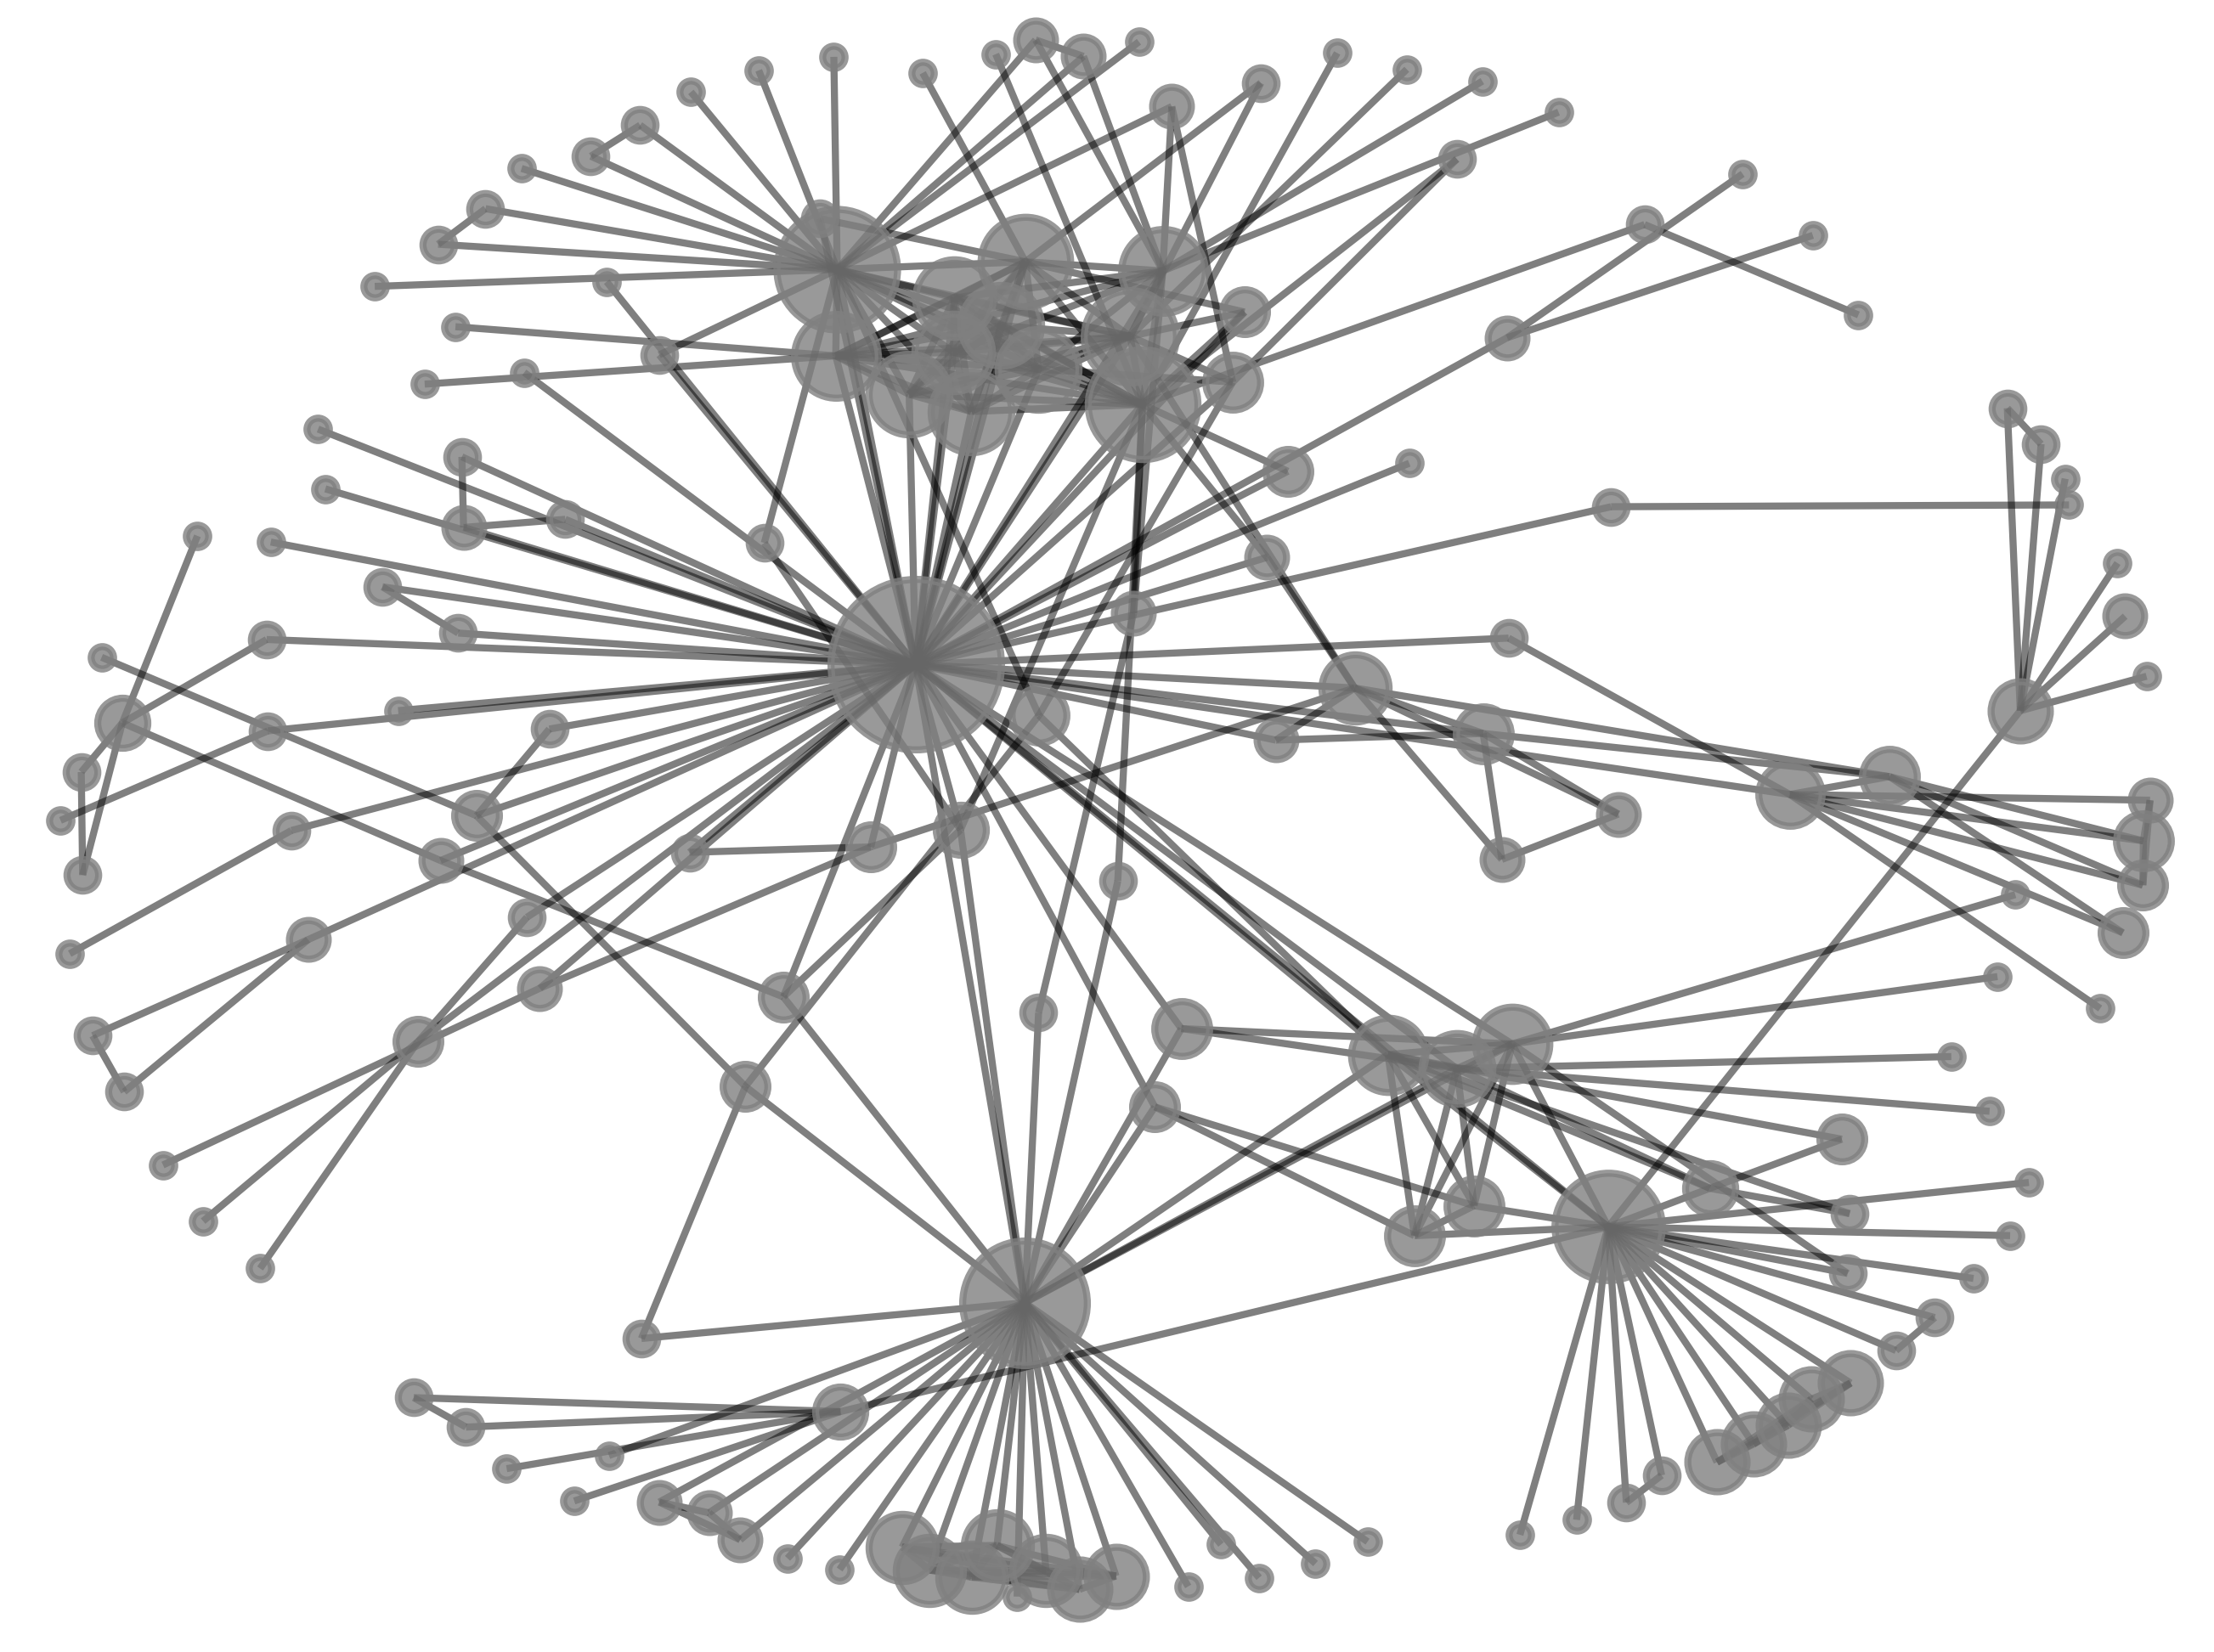
\includegraphics{OEIS/graph1}
\caption{Sequences network fetched by commands issued in the discussed session.}
\label{fig:oeis:sequences:network}
\end{figure}

\notbreakable{
    \inputminted[fontsize=\small,stripnl=false,firstline=31,lastline=44]
        {python}{deps/oeis-tools/src/graphing.py}
}

\notbreakable{
    \inputminted[fontsize=\small,stripnl=false,firstline=46,lastline=76]
        {python}{deps/oeis-tools/src/graphing.py}
}
